\documentclass[t,aspectratio=169]{beamer}

\usepackage{soul}
\usepackage{tikz}
\usepackage{multicol}
%\usepackage{gensymb}
\usepackage[utf8]{inputenc}

\usetikzlibrary{arrows.meta,decorations.markings}


%\usepackage{hyperref}
\hypersetup{
    colorlinks=true,
    linkcolor=blue,
    filecolor=magenta,      
    urlcolor=cyan,
    pdftitle={(KTXFI1EBNF) Physics I. Practice},
}

% ----------------------------------------------------------------------------------------------------------------------------------------

\title{\includegraphics[width=45pt]{oepecsetlogo.png}\\(KTXFI1EBNF) Physics I. Practice}

\author{Dr.~Gábor FACSKÓ, PhD\\\tiny Assistant Professor / Senior Research Fellow\\\textit{facsko.gabor@uni-obuda.hu}}

\institute{\Tiny Óbuda University, Faculty of Electrical Engineering, 1084 Budapest, Tavaszmező u. 17.\\Wigner Research Centre for Physics, Department of Space Physics and Space Technology, 1121 Budapest, Konkoly-Thege Miklós út 29–33.\\ \url{https://wigner.hu/~facsko.gabor}}

\date{March~30,~2026}

\logo{\includegraphics[height=0.9 true cm]{kekcsik.png}}

% ----------------------------------------------------------------------------------------------------------------------------------------

\begin{document}

\frame{\titlepage}

% ----------------------------------------------------------------------------------------------------------------------------------------

\begin{frame}[fragile,squeeze,allowframebreaks]
\frametitle{Exercises}
\begin{itemize}
\setlength{\parskip}{0pt}
\setlength{\itemsep}{0pt}
\item \textbf{Thermodynamics I:} Temperature scales, thermal expansion, thermometers. State variables, ideal gas, state changes, ideal gas equation of state, Boyle’s law, Gay-Lussac’s laws, universal (combined) gas law, heat, specific heat, molar heat, heat capacity.
\item \textbf{Thermodynamics II:} Expansion work, internal energy, the first law of thermodynamics, forms of the first law in different state changes.
\item \textbf{Thermodynamics III:} Cyclic processes, Carnot cycle, Carnot’s theorem, reduced heat, entropy, the second law of thermodynamics.
\item \textbf{Thermodynamics IV:} Kinetic theory of gases, molecular thermodynamics. Distributions, distribution functions. Elementary statistics.
  
\pagebreak
\item Problems:
\begin{enumerate}
\setcounter{enumi}{9}   
\item With air, whose initial pressure is $10^5\,Pa$ and temperature is $27^{\circ}C$, we perform the following cycle: We isothermally expand the gas to four times its original volume, then decrease its volume at constant pressure to the original value, and finally return it to its original state. What is the efficiency of the cycle?

\pagebreak
\item What is the efficiency of the cycle shown in the diagram if it is performed with a two-atomic (diatomic) molecule gas and $\frac{V_{2}}{V_{1}}$ = 2?
\begin{center}
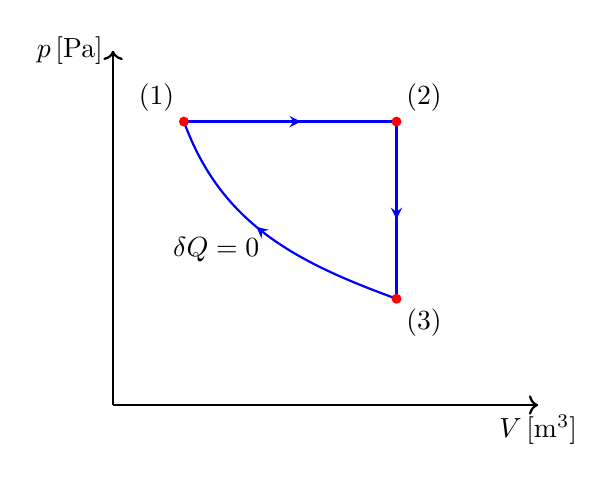
\begin{tikzpicture}[
    % Stílus a vonalak közepén elhelyezett nyilakhoz
    arrow inside/.style={
        postaction={decorate},
        decoration={
            markings,
            mark=at position 0.55 with {\arrow{stealth}}
        }
    }
,scale=0.9]

    % Tengelyek rajzolása feketével, nyilakkal a végén
    \draw[thick, ->] (0,0) -- (6,0) node[below] {$V \, [\mathrm{m^3}]$};
    \draw[thick, ->] (0,0) -- (0,5) node[left] {$p \, [\mathrm{Pa}]$};

    % Pontok koordinátáinak definiálása
    % (1): p=4, V=1
    % (2): p=4, V=4 (izobár 1-2)
    % (3): p=1.5, V=4 (izochor 2-3)
    \coordinate (P1) at (1,4);
    \coordinate (P2) at (4,4);
    \coordinate (P3) at (4,1.5);

    % Folyamatok rajzolása kékkel, középen nyíllal
    % 1 -> 2: Izobár (vízszintes)
    \draw[blue, thick, arrow inside] (P1) -- (P2);
    
    % 2 -> 3: Izochor (függőleges)
    \draw[blue, thick, arrow inside] (P2) -- (P3);
    
    % 3 -> 1: Adiabata (görbe)
    % A plot függvényt használjuk egy egyszerű hatványfüggvény modellezésére
    \draw[blue, thick, arrow inside] (P3) to[out=160, in=290] (P1);

    % Piros pontok és feliratok
    \fill[red] (P1) circle (2pt) node[above left, black] {(1)};
    \fill[red] (P2) circle (2pt) node[above right, black] {(2)};
    \fill[red] (P3) circle (2pt) node[below right, black] {(3)};

    % Adiabata feliratozása
    \node[black, left] at (2.2, 2.2) {$\delta Q = 0$};
\end{tikzpicture}
\end{center}

\pagebreak

\item The ideal cycle of an externally heated heat engine, shown in the diagram, differs from the Otto engine cycle in that it contains isothermal processes instead of adiabatic ones.
\vskip -10 pt
\begin{columns}
\begin{column}{0.3\textwidth}
\begin{center}
\vskip -10 pt
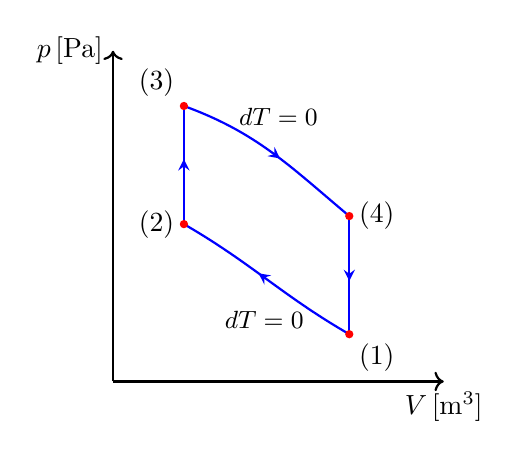
\begin{tikzpicture}[
    % Stílus a vonalak közepén elhelyezett nyilakhoz
    arrow inside/.style={
        postaction={decorate},
        decoration={
            markings,
            mark=at position 0.55 with {\arrow{stealth}}
        }
    }
,scale=0.6]

    % Tengelyek rajzolása feketével, nyilakkal a végén
    \draw[thick, ->] (0,0) -- (7,0) node[below] {$V \, [\mathrm{m^3}]$};
    \draw[thick, ->] (0,0) -- (0,7) node[left] {$p \, [\mathrm{Pa}]$};

    % Pontok koordinátáinak meghatározása
    % Úgy állítjuk be, hogy p3-p2 = p4-p1 legyen (ugyanakkora függőleges szakaszok)
    
    \coordinate (P1) at (5, 1);     % (1) Jobb alsó
    \coordinate (P2) at (1.5, 3.33); % (2) Balra fent (izoterma 1: p*V=5)
    \coordinate (P3) at (1.5, 5.83); % (3) Izochor (p3 = p2 + 2.5)
    \coordinate (P4) at (5, 3.5);    % (4) Izochor (p4 = p1 + 2.5), így p4-p1 = 2.5
    % Megjegyzés: A (3)-(4) görbe így egy másik izoterma (p*V = 1.5*5.83 = 8.75 és 5*3.5 = 17.5)
    % A fizikai hűség kedvéért a (3)-(4) ív is izotermikus marad a rajzon.

    % Folyamatok rajzolása kékkel, középen nyíllal
    % (1) -> (2): Izoterma (dT=0)
    \draw[blue, thick, arrow inside] (P1) to[out=150, in=330] (P2);
    
    % (2) -> (3): Izochor (függőleges, bal oldali)
    \draw[blue, thick, arrow inside] (P2) -- (P3);
    
    % (3) -> (4): Izoterma (dT=0)
    \draw[blue, thick, arrow inside] (P3) to[out=340, in=140] (P4);
    
    % (4) -> (1): Izochor (függőleges, jobb oldali, zárja a kört)
    \draw[blue, thick, arrow inside] (P4) -- (P1);

    % Piros pontok és címkék
    \fill[red] (P1) circle (2.5pt) node[below right, black] {(1)};
    \fill[red] (P2) circle (2.5pt) node[left, black] {(2)};
    \fill[red] (P3) circle (2.5pt) node[above left, black] {(3)};
    \fill[red] (P4) circle (2.5pt) node[right, black] {(4)};

    % Feliratok: dT=0 feketével az izotermák mellett
    \node[black, font=\small] at (3.2, 1.3) {$dT=0$}; 
    \node[black, font=\small] at (3.5, 5.6) {$dT=0$};
\end{tikzpicture}
\end{center}
\end{column}
\begin{column}{0.3\textwidth}
\vfill
What is the efficiency of the cycle if $p_{3} = 4 p_{2}$ , the compression ratio is 6, and the cycle is performed with a two-atomic (diatomic) gas? What is the efficiency of the Carnot cycle taking place between the same temperature limits?
\end{column}
\end{columns}
\end{enumerate}

\end{itemize}

\end{frame}

% ----------------------------------------------------------------------------------------------------------------------------------------

\begin{frame}
%\frametitle{Minden jó, ha a vége jó}

\vfill
\begin{center}
\textbf{\huge The End}

\bigskip
Thank you for your attention!
\end{center}
\vfill
%\textbf{Acknowledgements} Thank you for the course materials for Szilárd~ZSÓKA and Zoltán~VARGA.
\end{frame}

\end{document}
